\documentclass[11pt]{article}

\usepackage{mathtools}

\usepackage{float}
\usepackage{amssymb}
\usepackage{amsmath}
\usepackage{amsthm}
\usepackage{hyperref}
\usepackage{microtype}
\usepackage{graphicx}
\usepackage{blkarray}
\usepackage{pgfplots}
\pgfplotsset{compat=1.15}
\usepackage{mathrsfs}
\usetikzlibrary{arrows}
\graphicspath{ {./img/} }

\setlength{\parindent}{0cm}
\let\emptyset\varnothing

\title{\textbf{CSCI/MATH 2113 Discrete Structures} \\ Chapter 7 Relations The Second Time Around}
\author{Alyssa Motas}

\begin{document}

    \maketitle

    \pagebreak

    \tableofcontents

    \pagebreak

    \section{7.1 Properties of Relations}

    \subsection{Recall: Binary Relation}

    For sets $A, B$, any subset of \(A \times B\) is called a (\emph{binary}) \emph{relation} from $A$ to $B$. Any subset of \(A \times A\) is called a (\emph{binary}) \emph{relation} on $A$.

    \subsection{Properties of Relations}

    \subsubsection{Reflexive property}

    A relation $R$ on a set $A$ is called \emph{reflexive} if for all \(x \in A\), \((x,x) \in R\). This means that each element $x$ of $A$ is related to itself. 

    \vspace{1em}

    \emph{Example.} For \(A = \{1,2,3\}\) and \(R = \{(1,1), (1,2), (1,3), (2,2), (2,3)\}\), we know it is not reflexive since \((3,3) \notin R\).

    \vspace{1em}

    \emph{Remark.} A relation $R$ on $A$ is reflexive if and only if \(\{(a,a) \mid a \in A\} \subseteq R\).

    \vspace{1em}

    \emph{Counting.} Let $A$ be a set with $n$ elements. How many relations on $A$ are reflexive? There are \(2^{n^2}\) relations on $A$ (2 choices for each of the $n^2$ pairs in $A \times A$). In a reflexive relation, $n$ of these pairs are decided. Hence, we have \(n^2 - n\) chocies to make and so there are  \[2^{n^2 - 2}\] reflexive relations.

    \subsubsection{Symmetric property}

    A relation $R$ on a set $A$ is called \emph{symmetric} if \((x,y) \in R \Rightarrow (y,x) \in R\), for all, \(x,y \in A\).

    \vspace{1em}

    \emph{Counting.} If \(|A| = n \leq 0\), how many relations on $A$ are symmetric? Write \(A \times A = A_1 \cup A_2\) where
    \begin{align*}
        A_1 &= \{(a_i, a_i) \mid 1 \leq i \leq n\} \\
        A_2 &= \{(a_i, a_j) \mid 1 \leq i, j \leq n, i \neq j\}.
    \end{align*}
    We have \[|A_1| = n \qquad |A_2| = n^2 - n.\] For each element of \(A_1\) and for half of the elements of \(A_2\), we choose whether it belongs to $R$. Thus, intotal, there are \[2^n \cdot 2^{\frac{n^2-n}{2}} = 2^{\frac{n^2+n}{2}}\] such relations. In counthing those relations on $A$ that are both reflexive and symmetric, we have only one choice for each ordered pair in \(A_1\). So we have \[2^{\frac{n^2 - n}{2}}\] relations on $A$ that are both reflexive and symmetric.

    \subsubsection{Transitive property}

    For a set $A$, a relation $R$ on $A$ is called \emph{transitive} if, for all \(x,y,z \in A, (x,y), (y,z) \in R \Rightarrow (x,z) \in R\). So if $x$ ``is related to'' $y$, and $y$ ``is related to'' $z$, we want $x$ ``related to'' $z$, with $y$ playing the role of ``intermediary.''

    \vspace{1em}

    \emph{Counting.} There is no known general formula for the total number of transitive relations on a finite set.

    \subsubsection{Antisymmetric property}

    Given a relation $R$ on a set $A$, $R$ is called \emph{antisymmetric} if for all \(a,b \in A\), (\(a R b\) and \(b R a\)) \(\Rightarrow a = b.\) Here, the only way we can have both $a$ ``related to'' $b$ and $b$ ``related to'' $a$ is if $a$ and $b$ are one and the same element from $A$.

    \vspace{1em}

    \emph{Examples.} Let \(A = \mathbb{Z}\) and \(R = \leq\) is an antisymmetric relation.

    \vspace{1em}

    Antisymmetric is different than ``not symmetric.'' Let \(A = \{1,2,3\}\) and \(R = \{(1,2), (2,1), (2,3)\}\). Then, $R$ is \emph{not} symmetric and it is \emph{not} antisymmetric.

    \vspace{1em}

    \emph{Counting.} How relations that are antisymmetric? Suppose that \(|A| = n > 0\). By the rule of product, the number of antisymmetric relations are \[(2^n)(3^{\frac{n^2-n}{2}}).\]

    \subsection{Partial order}

    A relation $R$ on a set $A$ is called a \emph{partial order}, or a \emph{partial ordering relation}, if $R$ is reflexive, antisymmetric, and transitive.

    \subsubsection{Example}

    \begin{itemize}
        \item \(\leq\) on \(\mathbb{N}\). Partial order and total implies total order.
        \item \(\subseteq\) on \(\mathcal{P}(S)\) is not total order.
    \end{itemize}

    \subsection{Total order}

    A relation $R$ on a set $A$ is a \emph{total order} if $R$ is a partial order and for every \(x,y \in A,\) we have \((x,y) \in R\) or \((y,x) \in R\).

    \subsection{Equivalence relation}

    An \emph{equivalence relation} on $A$ is a relation that is reflexive, symmetric, and transitive.

    \section{7.2 Zero-One Matrices and Directed Graphs}
    
    \subsection{Relation Composition}

    If \(A,B\) and $C$ are sets with \(R_1 \subseteq A \times B\) and \(R_2 \subseteq B \times C\), then the \emph{composite relation} \(R_1 ; R_2\) is a relation from $A$ to $C$ defined by \[R_1 ; R_2 = \{(x,z) \mid x \in A, z \in C, \exists y \in B \text{ with } (x,y) \in R_1, (y,z) \in R_2\}.\]

    \subsubsection{Example}

    Suppose that \(A = \{1,2,3,4\}\), \(B = \{w,x,y,z\}\), and \(C = \{5,6,7\}\) where
    \begin{align*}
        R_1 &= \{(1,x),(2,x),(3,y),(3,z)\} \subseteq A \times B \\
        R_2 &= \{(w,5),(x,6)\} \subseteq B \times C \\
        R_3 &= \{(w,5), (w,6)\} \subseteq B \times C
    \end{align*}
    Then we have \[R_1;R_2 = \{(1,6),(2,6)\}\] and \[R_1;R_3 = \emptyset.\]

    \subsubsection{Theorem}

    Let \(A,B,C\) and $D$ be sets with \(R_1 \subseteq A \times B\), \(R_2 \subseteq B \times C\), and \(R_3 \subseteq C \times D.\) Then \(R_1;(R_2;R_3) = (R_1;R_2);R_3.\)

    \begin{proof}
        If \((a,d) \in R_1;(R_2;R_3)\), then there is an element \(b \in B\) with \((a,b) \in R_1\) and \((b,d) \in (R_2;R_3)\). Also, \((b,d) \in (R_2;R_3) \Rightarrow (b,c) \in R_2\) and \((c,d) \in R_3\) for some \(c \in C\). Then \((a,b) \in R_1\) and \((b,c) \in R_2 \Rightarrow (a,c) \in R_1;R_2\). Finally, \((a,c) \in R_1;R_2\) and \((c,d) \in R_3 \Rightarrow (a,d) \in (R_1;R_2);R_3\), and \(R_1;(R_2;R_3) \subseteq (R_1;R_2);R_3\). The opposite inclusion follows by similar reasoning.
    \end{proof}

    \subsubsection{Powers of a relation}

    Given a set $A$ and a relation $R$ on $A$, we define the \emph{powers} of $R$ recursively by 
    \begin{enumerate}
        \item[(a)] \(R^1 = R;\)
        \item[(b)] for \(n \in \mathbb{Z}^+, R^{n+1} = R;R^n.\)  
    \end{enumerate}

    \emph{Example.} Suppose that \(A = \{1,2,3,4\}\) and \(R = \{(1,2),(1,3),(2,4),(3,2)\}\). Then we have
    \begin{align*}
        R^2 &= \{(1,4),(1,2),(3,4)\} \\
        R^3 &= \{(1,4)\} \\
        R^n &= \emptyset \text{ for } n \leq 4.
    \end{align*}

    \subsection{Zero-one matrices}

    An \(m \times n\) \emph{zero-one matrix} \(E = (e_{ij})_{m \times n}\) is a rectangular array of numbers arranged in $m$ rows and $n$ columns, where each \(e_{ij}\), for \(1 \leq i \leq m\) and \(1 \leq j \leq n\), denotes the entry in the $i$th row and $j$th column of $E$, and each such entry is 0 or 1. 
    
    \vspace{1em}

    \emph{Example.} The matrix 
    \begin{equation*}
        E = \begin{bmatrix}
            1 & 0 & 0 & 1 \\
            0 & 1 & 0 & 1 \\
            1 & 0 & 0 & 0
        \end{bmatrix}
    \end{equation*}
    is a \(3 \times 4\) (0,1)-matrix where, for example, \(e_{11} = 1, e_{23} = 0,\) and \(e_{31} = 1.\)

    \vspace{1em}

    \(0\) is the matrix such that \(0_{i,j} = 0.\) And \(1\) is the matrix such that \(1_{i,j} = 1.\) \(I_n\) is the identity matrix where 
    \begin{equation*}
        (I_n)_{i,j} = S_{i,j} = \begin{cases}
            1 \quad \text{ if } i = j \\ 0 \quad \text{ if } i \neq j
        \end{cases}
    \end{equation*}

    If $M$ is a matrix then \(M^{tr}\) is \[(M^{tr})_{i,j} = M_{j,i}\]

    We think of 0 and 1 as truth values and of \(\cdot\) (multiplication) as conjunction and of + (addition) as disjunction. This means that
    \begin{align*}
        0 \cdot 0 = 0 && 0 + 0 = 0 \\
        0 \cdot 1 = 0 && 0 + 1 = 1 \\
        1 \cdot 0 = 0 && 1 + 0 = 1 \\
        \underbrace{1 \cdot 1 = 1}_\text{logical ``and''} && \underbrace{1 + 1 = 1}_\text{logical ``or''}
    \end{align*}

    We use these operations when multiplying matrices.

    \vspace{1em}

    \emph{Example.}

    \begin{align*}
        &\begin{bmatrix}
            0 & 1 \\ 1 & 0
        \end{bmatrix} \begin{bmatrix}
                        0 & 1 \\ 1 & 0
                      \end{bmatrix} = \begin{bmatrix}
                                        1 & 0 \\ 0 & 1
                                    \end{bmatrix} = I_2 \\
        &\begin{bmatrix}
            1 & 1 \\ 1 & 0
        \end{bmatrix} \begin{bmatrix}
                        1 & 0 \\ 1 & 0
                    \end{bmatrix} = \begin{bmatrix}
                                    1 & 0 \\ 1 & 0
                                \end{bmatrix}
    \end{align*}
    As well as multiplication, we define another operation on matrices.

    Let $M$ and $N$ be \((0,1)\)-matrices of the same size. Then \(M \cap N\) is defined as \[(M \cap N)_{i,j} = M_{i,j} \cdot N_{i,j}.\]

    \vspace{1em}

    \emph{Example.}
    \begin{equation*}
        \begin{bmatrix}
            1 & 0 \\ 1 & 0
        \end{bmatrix} \cap \begin{bmatrix}
                                1 & 1 \\ 0 & 0
                            \end{bmatrix} = \begin{bmatrix}
                                                1 & 0 \\ 0 & 0
                                            \end{bmatrix}
    \end{equation*}
 
    \vspace{1em}

    Let $M$ and $N$ be \((0,1)\)-matrices of the same size. Then \[M \leq N\] if \(M_{i,j} \leq N_{i,j}\) for all \(i,j\). In this case, we say that $M$ \emph{precedes} $N$.

    \vspace{1em}

    \emph{Examples.}
    \begin{align*}
        \begin{bmatrix}
            1 & 0 \\ 0 & 0
        \end{bmatrix} &\leq \begin{bmatrix}
                                1 & 1 \\ 0  & 0
                            \end{bmatrix} \\
        \begin{bmatrix}
            1 & 0 \\ 0 & 0
        \end{bmatrix} &\nleq \begin{bmatrix}
                                0 & 0 \\ 0 & 1
                            \end{bmatrix} \\
        \begin{bmatrix}
            1 & 0 \\ 0 & 0
        \end{bmatrix} &\ngeq \begin{bmatrix}
                                0 & 0 \\ 0 & 1
                            \end{bmatrix}
    \end{align*}

    \subsubsection{Relation matrices}

    Suppose we have \(A = \{1,2,3,4\}\), \(B = \{w,x,y,z\}\), \(C = \{5,6,7\}\), \(R_1 = \{(1,x),(2,x),(3,y),(3,z)\}\), and \(R_2 = \{ (w,5), (x,6) \}\). The matrix for \(R_1, R_2\) is

    \begin{equation*}
        M(R_1) = \begin{blockarray}{ccccc}
                    & w & x & y & z \\
                    \begin{block}{c[ cccc ]}
                        1 & 0 & 1 & 0 & 0 \\
                        2 & 0 & 1 & 0 & 0 \\
                        3 & 0 & 0 & 1 & 1 \\
                        4 & 0 & 0 & 0 & 0 \\
                    \end{block}
                \end{blockarray} \qquad M(R_2) = \begin{blockarray}{cccc}
                    & 5 & 6 & 7 \\
                    \begin{block}{c [ccc]}
                        w & 1 & 0 & 0 \\
                        x & 0 & 1 & 0 \\
                        y & 0 & 0 & 0 \\
                        z & 0 & 0 & 0 \\
                    \end{block}
                \end{blockarray}
    \end{equation*}
    We have \[M(R_1;R_2) = M(R_1) \cdot M(R_2).\] So to figure out what the matrix for \(R_1;R_2\) is, it suffices to multiply the matrices for \(R_1\) and \(R_2\).

    \begin{equation*}
        M(R_1;R_2) = \begin{bmatrix}
                        0 & 1 & 0 & 0 \\
                        0 & 1 & 0 & 0 \\
                        0 & 0 & 1 & 1 \\
                        0 & 0 & 0 & 0
                    \end{bmatrix} \cdot \begin{bmatrix}
                                            1 & 0 & 0 \\
                                            0 & 1 & 0 \\
                                            0 & 0 & 0 \\
                                            0 & 0 & 0
                                        \end{bmatrix} = \begin{bmatrix}
                                                            0 & 1 & 0 \\
                                                            0 & 1 & 0 \\
                                                            0 & 0 & 0 \\
                                                            0 & 0 & 0
                                                        \end{bmatrix}
    \end{equation*}

    \subsection{Theorem}

    Let $A$ be a set with \(|A| = n \leq 1\), $R$ be a relation on $A$, and $M$ be the matrix for $R$. Then 
    \begin{enumerate}
        \item $R$ is reflexive if and only if \(I_n \leq M\).
        \item $R$ is symmetric if and only if \(M = M^{tr}\).
        \item $R$ is transitive if and only if \(M^2 \leq M\).
        \item $R$ is antisymmetric if and only if \(M \cap M^{tr} \leq I_n\).
    \end{enumerate}

    \subsection{Directed graphs}

    Let $V$ be a finite nonempty set. A \emph{directed graph} (or \emph{digraph}) $G$ on $V$ is made up of the elements of $V$, called \emph{vertices} or \emph{nodes} of $G$, anda  subset $E$, of \(V \times V\), that contains the (\emph{directed}) \emph{edges}, or \emph{arcs}, of $G$. The set $V$ is called the \emph{vertex set} of $G$, and the set $E$ is called the \emph{edge set}. We then write \(G = (V,E)\) to denote the graph.

    \vspace{1em}

    If \(a,b \in V\) and \((a,b) \in E\), then there is an edge from $a$ to $b$. Vertex $a$ is called the \emph{origin} or \emph{source} of the edge, with $b$ the \emph{terminus}, or \emph{terminating vertex}, and we say that $b$ is \emph{adjacent from a} and that $a$ is \emph{adjacent} to $b$. In addition, if \(a \neq b\), then \((a,b) \neq (b,a).\) An edge of the form \((a,a)\) is called a \emph{loop} at $a$.

    \pagebreak

    \emph{Example.} Suppose that \(V = \{1,2,3,4,5\}\) and \(E = \{(1,1),(1,2),(1,4),(3,2)\}\). Then
    \begin{center}
        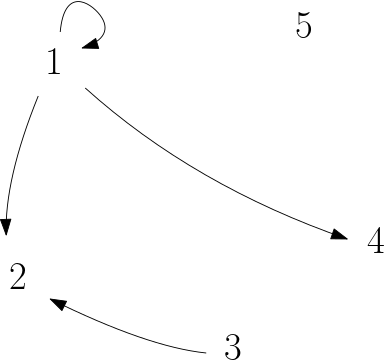
\includegraphics[width=5cm]{graph1.png}
    \end{center}

    We can interpret a relation on a set $A$ as a directed graph.

    \vspace{1em}

    \emph{Example.} Suppose that \(A = \{1,2,3,4\}\) and \(R = \{(1,1),(1,2),(2,3),(3,2),(3,3),(3,4),(4,2)\}\). Then we have 

    \begin{center}
        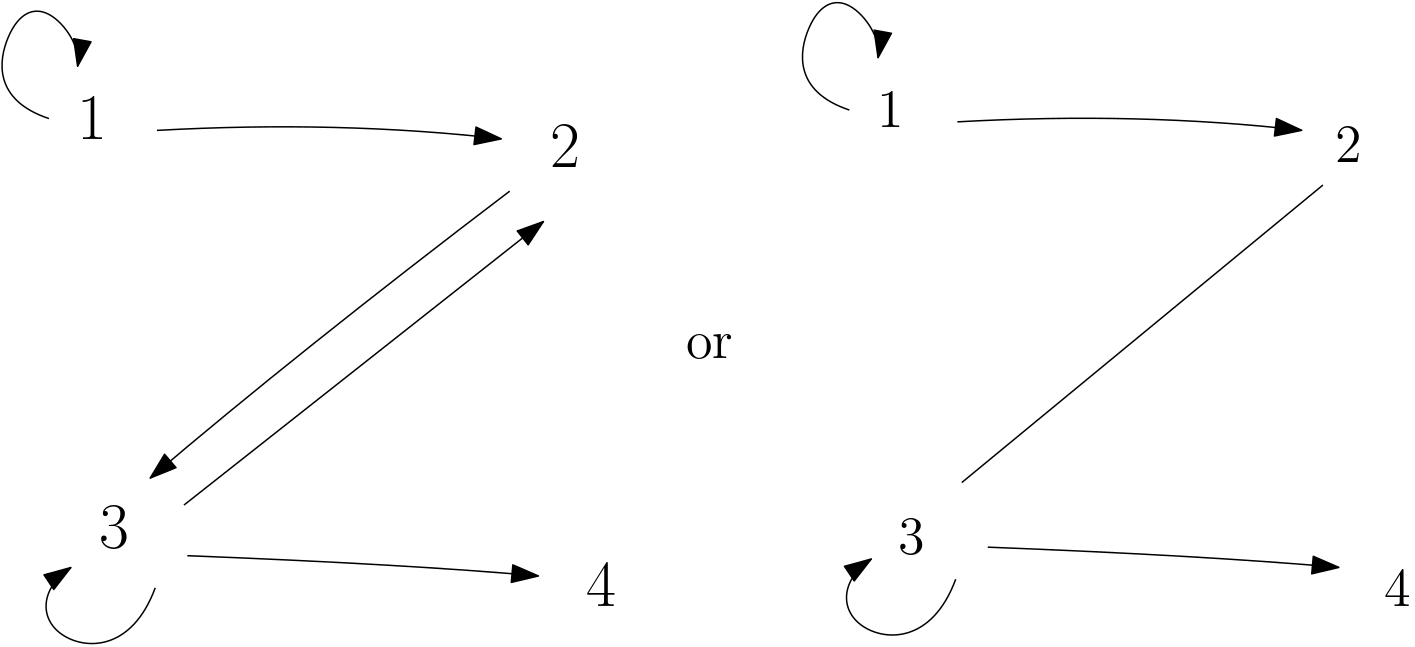
\includegraphics[width=10cm]{graph2.png}
    \end{center}

    The relation matrix $M$ is also called the adjacency matrix of the associated graph.

    \pagebreak

    \emph{Remark.} A relation is reflexive if and only if its directed graph has a loop at each vertex.

    \begin{center}
        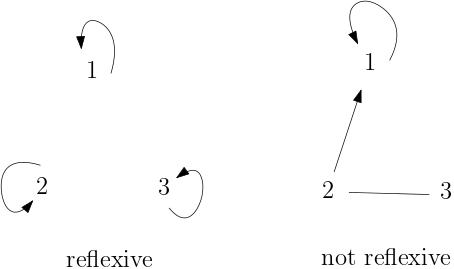
\includegraphics[width=7cm]{graph3.png}
    \end{center}

    \emph{Remark.} A relation is symmetric if and only if its directed graph contains only loops and undirected edges.

    \begin{center}
        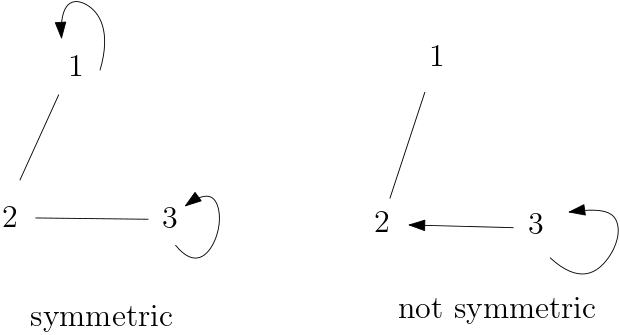
\includegraphics[width=7cm]{graph4.png}
    \end{center}

    \pagebreak

    \section{7.3 Partial Orders: Hasse Diagrams}

    A partial order on a set $A$ is a relation on $A$ that is reflexive, antisymmetric, and transitive.

    \vspace{1em}

    \emph{Example:} Let \(A = \{1,2,3,4\}\) and let $R$ be defined by \(xRy\) if and only if \(x \mid y\). Then we have \(R = \{(1,1),(2,2),(3,3),(4,4),(1,2),(1,3),(1,4),(2,4)\}\).
    \begin{figure}[H]
        \centering
        \begin{tikzpicture}[line cap=round,line join=round,>=triangle 45,x=1cm,y=1cm,scale=2]
            \clip(-1.075931722013576,0.2789242362804245) rectangle (6.1406798867869465,4.81521469272618);
            \draw [->,line width=1pt] (1.0162808377742203,1.0240821619049398) -- (1.9937796441609141,2.486599460010221);
            \draw [->,line width=1pt] (1.0162808377742203,1.0240821619049398) -- (0.04997476581180149,2.4567521682121543);
            \draw [->,line width=1pt] (1.0162808377742203,1.0240821619049398) -- (1.0061164051394844,3.7931512194088013);
            \draw [->,line width=1pt] (0.049974765811801505,2.4567521682121543) -- (1.0061164051394844,3.7931512194088013);
            \draw [line width=1pt] (4.190739153360531,0.9945586341425137)-- (5.09937959823203,2.325687948285471);
            \draw [line width=1pt] (4.190739153360531,0.9945586341425137)-- (3.235798558431886,2.487738473485483);
            \draw [line width=1pt] (3.235798558431886,2.487738473485483)-- (4.005538553131945,3.6799673374570014);
            \draw (0.3,4.3629988216786275) node[anchor=north west] {$\text{Directed Graph}$};
            \draw (3.5,4.3629988216786275) node[anchor=north west] {$\text{Hasse Diagram}$};
            \begin{scriptsize}
                \draw [fill=black] (1.0162808377742203,1.0240821619049398) circle (1.5pt);
                \draw[color=black] (1.1097783213829269,0.926629259916241) node {$A$};
                \draw [fill=black] (0.049974765811801505,2.4567521682121543) circle (1.5pt);
                \draw[color=black] (-0.006629610265717942,2.335093274949762) node {$B$};
                \draw [fill=black] (1.9937796441609141,2.486599460010221) circle (1.5pt);
                \draw[color=black] (2.0754476293490542,2.4057520048009424) node {$C$};
                \draw [fill=black] (1.0061164051394844,3.7931512194088013) circle (1.5pt);
                \draw[color=black] (1.123910067353163,3.734136126003126) node {$D$};
                \draw [fill=black] (4.190739153360531,0.9945586341425137) circle (1.5pt);
                \draw[color=black] (4.3082634926463435,0.8465493660849037) node {$E$};
                \draw [fill=black] (3.235798558431886,2.487738473485483) circle (1.5pt);
                \draw[color=black] (3.135328577116755,2.297408619029133) node {$F$};
                \draw [fill=black] (5.09937959823203,2.325687948285471) circle (1.5pt);
                \draw[color=black] (5.2032740707612914,2.226749889177953) node {$G$};
                \draw [fill=black] (4.005538553131945,3.6799673374570014) circle (1.5pt);
                \draw[color=black] (4.152814286973747,3.639924486201553) node {$H$};
            \end{scriptsize}
        \end{tikzpicture}
    \end{figure}

    If $R$ is a partial order on $A$ then we draw a line \emph{up} from $x$ to $y$ if \(xRy\) and there is no $z$ such that \(xRz\) and \(zRy\).

    \vspace{1em}

    \emph{Examples:}
    \begin{itemize}
        \item If \(A = \{1,2,4,8\}\) and $R$ is ``divides.''
        \begin{figure}[H]
            \centering
            \begin{tikzpicture}[line cap=round,line join=round,>=triangle 45,x=1cm,y=1cm]
                \clip(0.3813526482831465,0.5521782278604659) rectangle (3.2830316396300763,3.37614485231679);
                \draw (1.4628531078517475,1.7718876031843844) node[anchor=north west] {$1$};
                \draw (1.447700737139753,2.29653843908719) node[anchor=north west] {$2$};
                \draw (1.42876027374976,3.330687740180807) node[anchor=north west] {$8$};
                \draw (1.4382305054447566,2.7870964408880083) node[anchor=north west] {$4$};
                \draw [line width=1pt] (1.426369229651408,1.7144833676047389)-- (1.4155290342394133,2.232102698527485);
                \draw [line width=1pt] (1.4155290342394133,2.232102698527485)-- (1.4073988876804173,2.7172014432142473);
                \draw [line width=1pt] (1.4073988876804173,2.7172014432142473)-- (1.40197878997442,3.2754715069319738);
                \begin{scriptsize}
                \draw [fill=black] (1.426369229651408,1.7144833676047389) circle (2.5pt);
                \draw [fill=black] (1.4155290342394133,2.232102698527485) circle (2.5pt);
                \draw [fill=black] (1.4073988876804173,2.7172014432142473) circle (2.5pt);
                \draw [fill=black] (1.40197878997442,3.2754715069319738) circle (2.5pt);
                \end{scriptsize}
                \end{tikzpicture}
        \end{figure}
        \item If \(A = \{2,3,5,7\}\) and $R$ is ``divides.'' \[2 \quad 3 \quad 5 \quad 7\]
        \item If \(B = \{1,2,3\}\), \(A = \mathcal{P}(\{1,2,3\})\) and $R$ is \(\subseteq\).
        \begin{figure}[H]
            \centering
            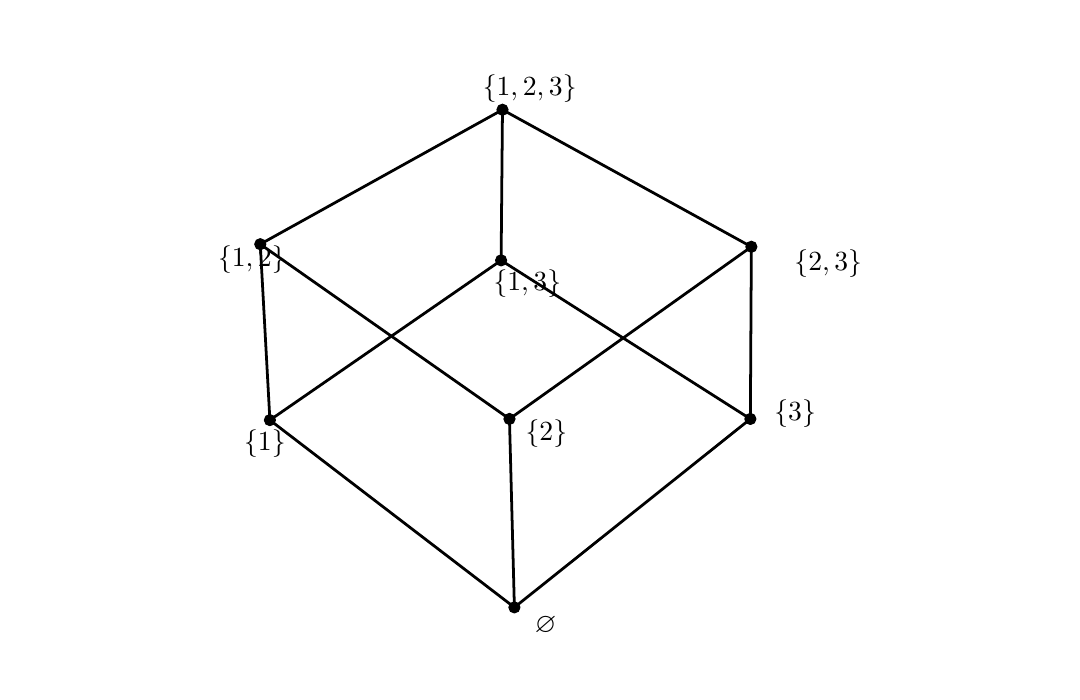
\begin{tikzpicture}[line cap=round,line join=round,>=triangle 45,x=1cm,y=1cm,scale=4]
                \clip(-0.12731603340699826,1.517730858292495) rectangle (3.1253230517932513,3.5623075156344184);
                \draw [line width=1pt] (0.641732829026252,2.31630567523753)-- (1.4180072775835197,1.7217278358356483);
                \draw [line width=1pt] (1.4180072775835197,1.7217278358356483)-- (2.16724,2.32);
                \draw [line width=1pt] (1.4180072775835197,1.7217278358356483)-- (1.40235,2.32);
                \draw [line width=1pt] (1.40235,2.32)-- (2.170376586506866,2.8666174279305494);
                \draw [line width=1pt] (0.641732829026252,2.31630567523753)-- (0.61116,2.8748);
                \draw [line width=1pt] (0.61116,2.8748)-- (1.40235,2.32);
                \draw [line width=1pt] (0.641732829026252,2.31630567523753)-- (1.3758618205889392,2.8234573840093);
                \draw [line width=1pt] (1.3758618205889392,2.8234573840093)-- (2.16724,2.32);
                \draw [line width=1pt] (0.61116,2.8748)-- (1.380185351870733,3.3016929589057997);
                \draw [line width=1pt] (1.380185351870733,3.3016929589057997)-- (2.170376586506866,2.8666174279305494);
                \draw [line width=1pt] (2.170376586506866,2.8666174279305494)-- (2.16724,2.32);
                \draw [line width=1pt] (1.380185351870733,3.3016929589057997)-- (1.3758618205889392,2.8234573840093);
                \draw (1.4522945928260211,1.7236747168201862) node[anchor=north west] {$\emptyset$};
                \draw (2.2123760500725544,2.4115696669539175) node[anchor=north west] {$\{3\}$};
                \draw (0.5287319282946187,2.316028701657566) node[anchor=north west] {$\{1\}$};
                \draw (1.422570736956045,2.3499988226518242) node[anchor=north west] {$\{2\}$};
                \draw (0.4459297583711136,2.899890156246381) node[anchor=north west] {$\{1,2\}$};
                \draw (1.3206603739732694,2.8255805165714407) node[anchor=north west] {$\{1,3\}$};
                \draw (2.276070026936789,2.887151360873534) node[anchor=north west] {$\{2,3\}$};
                \draw (1.286690252979011,3.443412092154514) node[anchor=north west] {$\{1,2,3\}$};
                \begin{scriptsize}
                \draw [fill=black] (1.4180072775835197,1.7217278358356483) circle (0.5pt);
                \draw [fill=black] (1.40235,2.32) circle (.5pt);
                \draw [fill=black] (0.641732829026252,2.31630567523753) circle (.5pt);
                \draw [fill=black] (2.16724,2.32) circle (.5pt);
                \draw [fill=black] (2.170376586506866,2.8666174279305494) circle (.5pt);
                \draw [fill=black] (0.61116,2.8748) circle (.5pt);
                \draw [fill=black] (1.3758618205889392,2.8234573840093) circle (.5pt);
                \draw [fill=black] (1.380185351870733,3.3016929589057997) circle (.5pt);
                \end{scriptsize}
                \end{tikzpicture}
        \end{figure}
    \end{itemize}

    \subsection{Totally ordered poset}

    If \((A,R)\) is a poset, we say that $A$ is \emph{totally ordered} (or, \emph{lineraly ordered}) if for all \(x,y \in A\) either \(xRy\) or \(yRx\). In this case $R$ is called \emph{total order} (or, a \emph{linear order}).

    \vspace{1em}

    \emph{Examples}
    \begin{itemize}
        \item \((\mathbb{Z}, \leq)\) is totally ordered.
        \item \((P(\{a,b\}), \subseteq)\) is not totally ordered. Indeed, \(\{a\} \not\subseteq \{b\}\) and \(\{b\} \not\subset \{a\}\).
    \end{itemize}

    \emph{Question:} Given a partially ordered set, can we ``extend'' this relation so that the order becomes total? YES: topological sorting.

    \subsection{Maximal and minimal}

    If \((A,R)\) is a psoet, then an element \(x \in A\) is called a \emph{maximal} element of $A$ if for all \(a \in A\), \(a \neq x \Rightarrow (x,a)\notin R\). An element \(y \in A\) is called \emph{minimal} elment of $A$ if whenever \(b \in A\) and \(b \neq y\), then \((b,y)\notin R\).

    \vspace{1em}

    \emph{Example:} Let \(A = \mathcal{P}(\{1,2,3\})\) and \(R = \subseteq\). Then \(\{1,2,3\}\) is the maximal element and \(\emptyset\) is the minimal element.

    \vspace{1em}

    Let $A$ be the collection of proper subsets of \(\{1,2,3\}\) ordered by inclusion. Then. \(\{1,2\}\) is a maximal element and so is \(\{2,3\}\). Recall: for $S$ and $T$ sets, we have \(S \subseteq T\) if \(\forall x, x \in S \Rightarrow x \in T.\)

    \subsection{Conditions for maximal and minimal element in a set}

    If \((A,R)\) is a nonempty poset and $A$ is finite, then $A$ has a maximal element and a minimal element.
    \begin{proof}
        Let \(a_1 \in A\). If there is no element \(a \in A\) where \(a \neq a_1\) and \(a_1 R a\), then \(a_1\) is maximal. Otherwise there is an element \(a_2 \in A\) with \(a_2 \neq a_1\) and \(a_1 R a_2\). If no element \(a \in A\), \(a \neq a_2\), satisfies \(a_2 R a\), then \(a_2\) is maximal. Otherwise we can find \(a_3 \in A\) so that \(a_3 \neq a_2\), \(a_3, \neq a_1\) while \(a_1 R a_2\) and \(a_2 R a_3\). Continuing in this manner, since $A$ is finite, we get to an element \(a_n in A\) with \((a_n, a) \notin R\) for all \(a \in A\) where \(a \neq a_n\), so \(a_n\) is maximal. The proof for a minimal element follows in a similar way.
    \end{proof}

    \subsection{Greatest and least element}

    If \((A,R)\) is a poset, then an element \(x \in A\) is called a \emph{least} element if \(x R a\) for all \(a \in A\). Element \(y \in A\) is called a \emph{greatest} element if \(aRy\) for all \(a \in A\).

    \vspace{1em}

    \emph{Examples}
    \begin{itemize}
        \item \((\mathcal{P}(\{1,2,3\}),\subseteq)\) has a maximal and a greatest element of \(\{1,2,3\}\).
        \item \((\mathcal{P}(\{1,2,3\}) \setminus \{\{1,2,3\}\}, \subseteq)\) has maximal elements (e.g., \(\{1,2\}\)) but no greatest element.
    \end{itemize}

    \subsection{Greatest and least elements are unique}

    If the poset \((A,R)\) has a greatest (least) element, then that element is unique.
    \begin{proof}
        Suppose that \(x,y \in A\) and that both are greatest elements. Since $x$ is a greatest element, \(yRx\). Likewise, \(xRy\) because $y$ is a greatest element. As $R$ is antisymmetric, it follows that \(x=y\). The proof for the least element is similar.
    \end{proof}

    \subsection{Lower and upper bounds}

    Let \((A,R)\) be a poset with \(B \subseteq A\). An element \(x \in A\) is called a \emph{lower bound} of $B$ if \(xRb\) for all \(b \in B\). Likewise, an element \(y \in A\) is called an \emph{upper bound} of $B$ if \(bRy\) for all \(b \in B\).

    An element \(x' \in A\) is called a \emph{greatest lower bound} (glb) of $B$ if it is a lower bound of $B$ and if for all other lower bounds \(x''\) of $B$ we have \(x'' R x'\). Similarly \(y' \in A\) is a \emph{least upper bound} (lub) of $B$ if it is an upper bound of $B$ and if \(y' R y''\) for all other upper bounds \(y''\) of $B$.

    \subsection{Unique lub/glb}

    If \(A,R\) is a poset and \(B \subseteq A\), then $B$ has at most one lub (glb).

    \subsection{Lattice}

    The poset \((A,R)\) is called a \emph{lattice} if for all \(x,y \in A\) the elements \(\text{lub}\{x,y\}\) and \(\text{glb}\{x,y\}\) both exist in $A$.

    \vspace{1em}

    \emph{Example:} Let $S$ be a set. Then \((\mathcal{P}(S),\subseteq)\) is a lattice.

    \section{7.4 Equivalence Relations and Partitions}

    Given a set $A$ and index set $I$, let \(\emptyset \neq A_i \subseteq A\) for each \(i \in I\). Then \(\{A_i\}_{i \in I}\) is a \emph{partition} of $A$ if 
    \begin{enumerate}
        \item[a)] \(A = \bigcup_{i \in I} A_i\) and
        \item[b)] \(A_i \cap A_j = \emptyset\) for all \(i,j \in I\) where \(i \neq j\).
    \end{enumerate}
    Each subset \(A_i\) is called a \emph{cell} or \emph{block} of the partition.

    \subsection{Examples}
    \begin{itemize}
        \item Let \(A = \{1,2, \dots, 10\} \subseteq \mathbb{Z}\). The following are partitions of $A$:
        \begin{enumerate}
            \item \(\{A_1, A_2\}\) where \[A_1 = \{1, \dots, 5\} \quad \text{and} \quad A_2 = \{6, \dots, 10\}.\]
            \item \(\{A_1, A_2, A_3\}\) where \[A_1 = \{1,2,3\}, \quad A_2 = \{4,5,6\}, \quad \text{and} \quad A_3 = \{7,8,9,10\}.\] 
            \item \(\{A_i\}_{1 \leq i \leq 5}\) where \[A_i = \{i, i+5\}.\]
        \end{enumerate}
        \item \(\{A_i\}_{i \in \mathbb{Z}}\) where \(A_i = [i, i+1) \subseteq R\) is a partition of \(\mathbb{R}\). 
    \end{itemize}

    \subsection{Equivalence class}

    Let $R$ be an equivalence relation on a set $A$. For each \(x \in A\), the \emph{equivalence class} of $x$, denoted \([x]\), is defined by \([x] = \{y \in A \mid y R x\}\). 
    
    \subsection{Example}

    Consider the relation \(\equiv_4\) on \(\mathbb{Z}\) defined by \[x \equiv_4 y \Leftrightarrow 4 \mid (x-y).\]
    \begin{itemize}
        \item \([0] = \{y \in \mathbb{Z} \mid y \equiv_4 = 0\} \Rightarrow \{y \in \mathbb{Z} \mid 4 \mid y\} \Rightarrow \{\dots, -8, -4, 0, 4 ,8, \dots\}\).
        \item \([1] = \{\dots, -3,1,5,9,\dots\}\).
        \item \([2] = \{\dots, -2, 2, 6,\dots\}\).
        \item \([3] = \{\dots, -5, -1, 3,7,\dots\}\).
    \end{itemize}

    \emph{Remark:} \(\{[0],[1],[2],[3]\}\) is a partition of \(\mathbb{Z}\). 

    \vspace{1em}

    \emph{Question:} Is this always the case? That is, if $R$ is an equivalence relation on $A$, does the collection of equivalence classes form a partition of $A$? Yes!

    \subsection{Equivalence relation}

    If $R$ is an equivlanece relation on a set $A$, and \(x,y \in A\) then 
    \begin{enumerate}
        \item[(a)] \(x \in [x]\);
        \item[(b)] \(xRy\) if and only if \([x] = [y]\);
        \item[(c)] \([x] = [y]\) or \([x] \cap [y] = \emptyset\).   
    \end{enumerate}

    \begin{proof}
        \begin{enumerate}
            \item[(a)] This result follows from the reflexive property of $R$.
            \item[(b)] If \(xRy\), let \(w \in [x]\). Then \(w  R x\) and because $R$ is transitive, \(w R y\). Hence \(w \in [y]\) and \([x] \subseteq [y]\). With $R$ symmetric, \(xRy \Rightarrow yRx\). So if \(t \in [y]\), then \(t R y\) and by the transitive property, \(t R x\). Hence \(t \in [x]\) and \([y] \subseteq [x]\). Consequently, \([x] = [y]\). Conversely, let \([x] = [y]\). Since \(x \in [x]\) by part (a), then \(x \in [y]\) or \(x R y\).   
            \item[(c)] This property tells us that two equivalence classes can be related in only one of two possible ways. Either they are idenitcal or they are disjoint.
            
            We assume that \([x] \neq [y]\) and show how it then follows that \([x] \cap [y] = \emptyset\). If \([x] \cap [y] \neq \emptyset\), then let \(v \in A\) with \(v \in [x]\) and \(v \in [y]\). Then \(v R x, v R y\), and, since $R$ is symmetric, \(x R v\). Now \((xRv \text{ and } v R y) \Rightarrow x R y\), by the transitive property. Also \(xRy \Rightarrow [x] = [y]\) by part (b). This contradicts the assumption that \([x] \neq [y]\), so we reject the supposition that \([x] \cap [y] \neq \emptyset\), and the result follows.
        \end{enumerate}
    \end{proof}

    \emph{Corollary:} If $R$ is an equivalence relation on $A$ then \[\{[x] \mid [x] \text{ is the equivalence class of } x\}\] is a partition of $A$. This tells us that some partition arise through equivalence relations. In fact, all partitions arise in this way!


    \subsection{Equivalence classes and partition}

    If $P$ is a partition of $A$ and \(R_p\) is defined as \[x R_p y \Leftrightarrow x \text{ and } y \text{ belong to the same cell of } A\] then $P$ consists of the equivalence classes of \(R_p\). 

    And for any set $A$, there is a one-to-one correspondence between the set of equivalence relations on $A$ and the set of partitions of $A$.


\end{document}